\documentclass[10pt]{beamer}
\usetheme[
%%% options passed to the outer theme
%    hidetitle,           % hide the (short) title in the sidebar
%    hideauthor,          % hide the (short) author in the sidebar
%    hideinstitute,       % hide the (short) institute in the bottom of the sidebar
%    shownavsym,          % show the navigation symbols
%    width=2cm,           % width of the sidebar (default is 2 cm)
%    hideothersubsections,% hide all subsections but the subsections in the current section
%    hideallsubsections,  % hide all subsections
    left               % right of left position of sidebar (default is right)
%%% options passed to the color theme
%    lightheaderbg,       % use a light header background
  ]{AAUsidebar}

% If you want to change the colors of the various elements in the theme, edit and uncomment the following lines
% Change the bar and sidebar colors:
%\setbeamercolor{AAUsidebar}{fg=red!20,bg=red}
%\setbeamercolor{sidebar}{bg=red!20}
% Change the color of the structural elements:
%\setbeamercolor{structure}{fg=red}
% Change the frame title text color:
%\setbeamercolor{frametitle}{fg=blue}
% Change the normal text color background:
%\setbeamercolor{normal text}{bg=gray!10}
% ... and you can of course change a lot more - see the beamer user manual.


\usepackage[utf8]{inputenc}
\usepackage[english]{babel}
\usepackage[T1]{fontenc}
% Or whatever. Note that the encoding and the font should match. If T1
% does not look nice, try deleting the line with the fontenc.
\usepackage{helvet}

% colored hyperlinks
\newcommand{\chref}[2]{%
  \href{#1}{{\usebeamercolor[bg]{AAUsidebar}#2}}%
}

\title[The effect of limb position on myoelectric prosthetic control using linear regression]% optional, use only with long paper titles
{The effect of limb position on myoelectric prosthetic control using linear regression}

\subtitle{Scientific Methods and Communication Conference 2017}  % could also be a conference name

\date{December 14, 2017}	%or use \today if today is today

\author[Group 7404] % optional, use only with lots of authors
{
  %Jesper Kjær Nielsen\\
  %\href{mailto:jkn@es.aau.dk}{{\tt jkn@es.aau.dk}}
  Irene Uriarte\\
  Martin Garenfeld\\
  Oliver Damsgaard\\
  Simon Bruun
}
% - Give the names in the same order as they appear in the paper.
% - Use the \inst{?} command only if the authors have different
%   affiliation. See the beamer manual for an example

\institute[
%  {\includegraphics[scale=0.2]{aau_segl}}\\ %insert a company, department or university logo
  School of Medicine and Health\\
  Aalborg University\\
  Denmark
] % optional - is placed in the bottom of the sidebar on every slide
{% is placed on the title page
  School of Medicine and Health\\
  Aalborg University\\
  Denmark
  
  %there must be an empty line above this line - otherwise some unwanted space is added between the university and the country (I do not know why;( )
}


% specify a logo on the titlepage (you can specify additional logos an include them in 
% institute command below
\pgfdeclareimage[height=1.5cm]{titlepagelogo}{AAUgraphics/aau_logo_new} % placed on the title page
%\pgfdeclareimage[height=1.5cm]{titlepagelogo2}{graphics/aau_logo_new} % placed on the title page
\titlegraphic{% is placed on the bottom of the title page
  \pgfuseimage{titlepagelogo}
%  \hspace{1cm}\pgfuseimage{titlepagelogo2}
}


\begin{document}
% the titlepage
{\aauwavesbg%
\begin{frame}[plain,noframenumbering] % the plain option removes the sidebar and header from the title page
  \titlepage
\end{frame}}
%%%%%%%%%%%%%%%%

% TOC
\begin{frame}{Agenda}{}
\tableofcontents
\end{frame}
%%%%%%%%%%%%%%%%

\section{Introduction}
% motivation for creating this theme
\begin{frame}{Introduction}{}
  \begin{itemize}
    \item Myoelectric prosthetics
    \vspace{4.5cm}
  \end{itemize}
\end{frame}

\begin{frame}{Introduction}{}
\begin{itemize}
	\item Myoelectric prosthetics
	\item Variations in limb positions lower accuracy [1]\\
	\vspace{3cm}
	[1] Fougner et al. IEEE TNSRE (2011)
\end{itemize}
\end{frame}

\begin{frame}{Introduction}{}
\begin{itemize}
	\item Myoelectric prosthetics
	\item Variations in limb positions lower accuracy [1]
	\item Classification [1] vs regression [2]\\
	\vspace{3cm}
	[1] Fougner et al. IEEE TNSRE (2011)
	
	[2] Hahne et al. IEEE TNSRE (2014)
\end{itemize}
\end{frame}

\begin{frame}{Introduction}{}
\begin{itemize}
	\item Myoelectric prosthetics
	\item Variations in limb positions lower accuracy [1]
	\item Classification [1] vs regression [2]
	\item Test performance of linear regression- based control across different limb positions\\
	\vspace{3cm}
	[1] Fougner et al. IEEE TNSRE (2011)
	
	[2] Hahne et al. IEEE TNSRE (2014)
\end{itemize}
\end{frame}


%%%%%%%%%%%%%%%%

%%% M&M %%%

\section{Methods and Materials}
% the license
\begin{frame}{Methods and Materials}

\end{frame}

%%% MOVEMENTS and LIMB POSITIONs %%%

\subsection{Data Acquisition}
\begin{frame}{Methods and Materials}{Wrist Movements}
  \begin{figure}
  		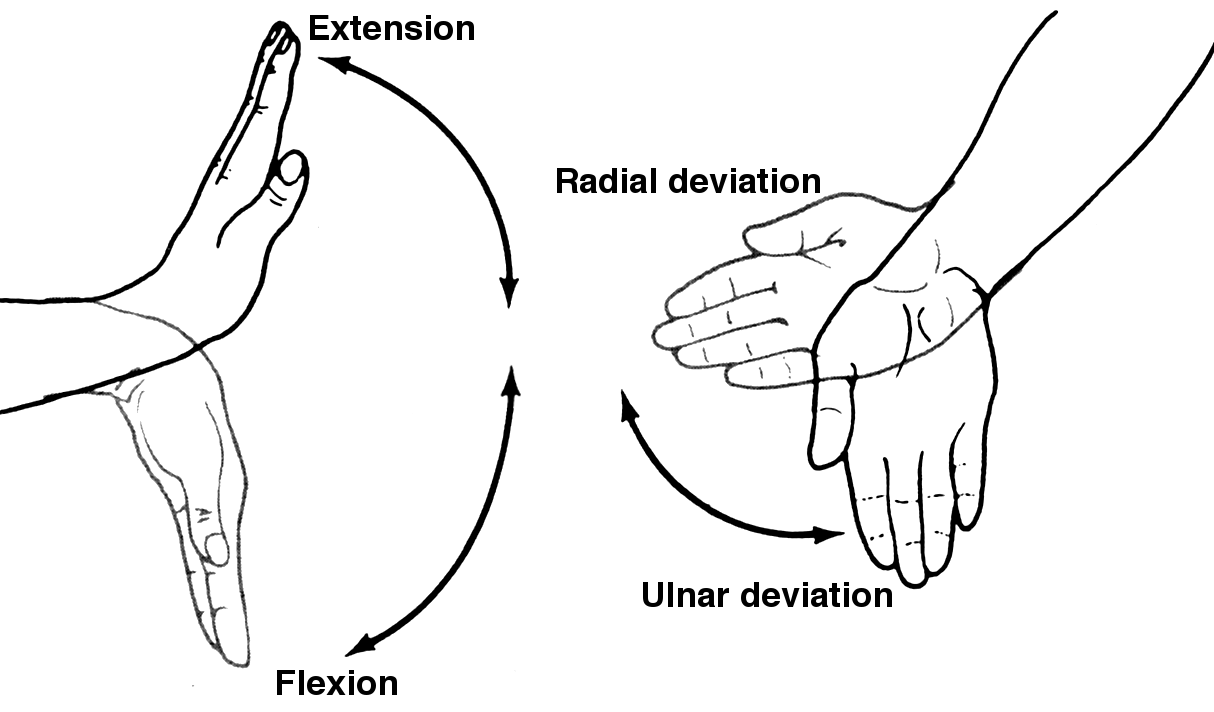
\includegraphics[scale=1]{figures/wrist_move.png}
  \end{figure}
\end{frame}

%%% GUI %%%

\subsection{GUI}
\begin{frame}{Methods and Materials}{Training GUI}
 \begin{figure}
 	\includegraphics[scale=0.225]{figures/GUI_training.png}
 \end{figure}
\end{frame}

%\subsection{GUI}
\begin{frame}{Methods and Materials}{Test GUI}
\begin{figure}
	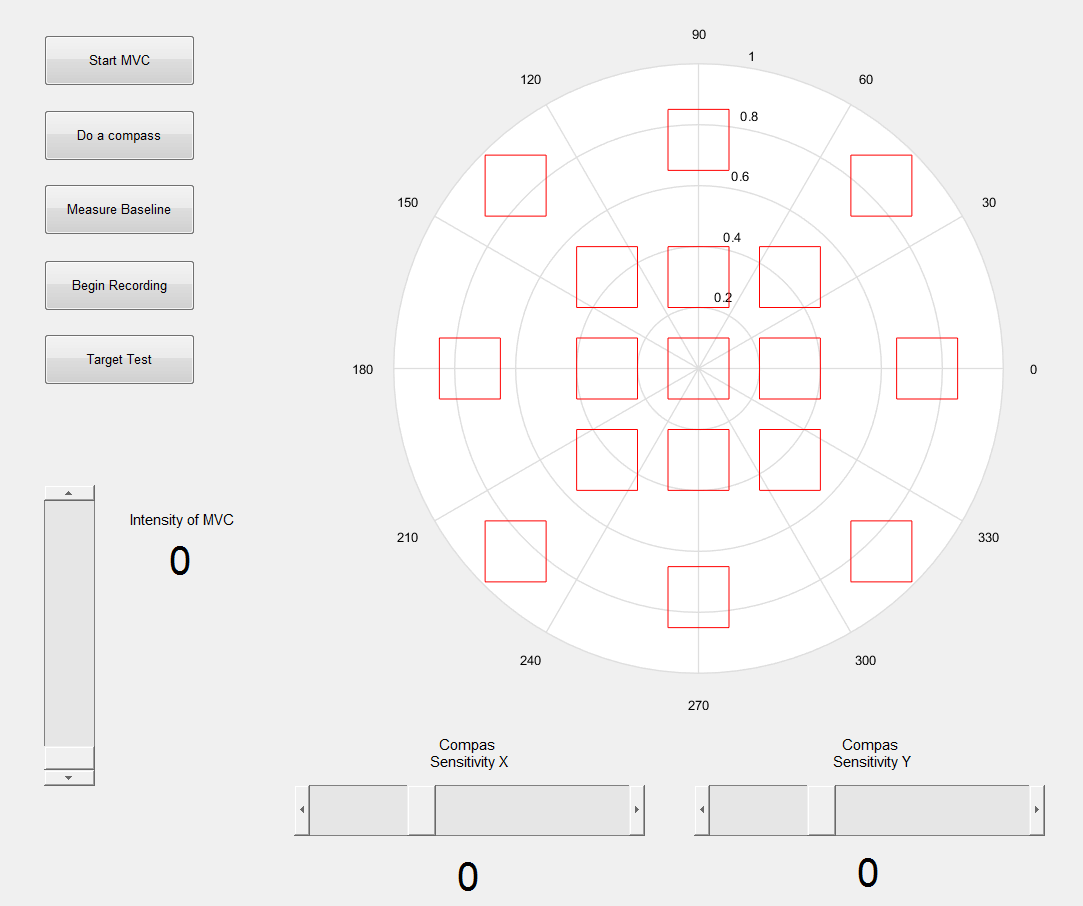
\includegraphics[scale=0.3]{figures/PlacesToGo.png}
\end{figure}
\end{frame}

%%% RESULTS %%%

\section{Results}
% the license
\begin{frame}{Results}

\end{frame}

%%% Offline results %%%

\subsection{Offline Results}
	\begin{frame}{Results}{Offline Results: training data}
		\begin{figure}
			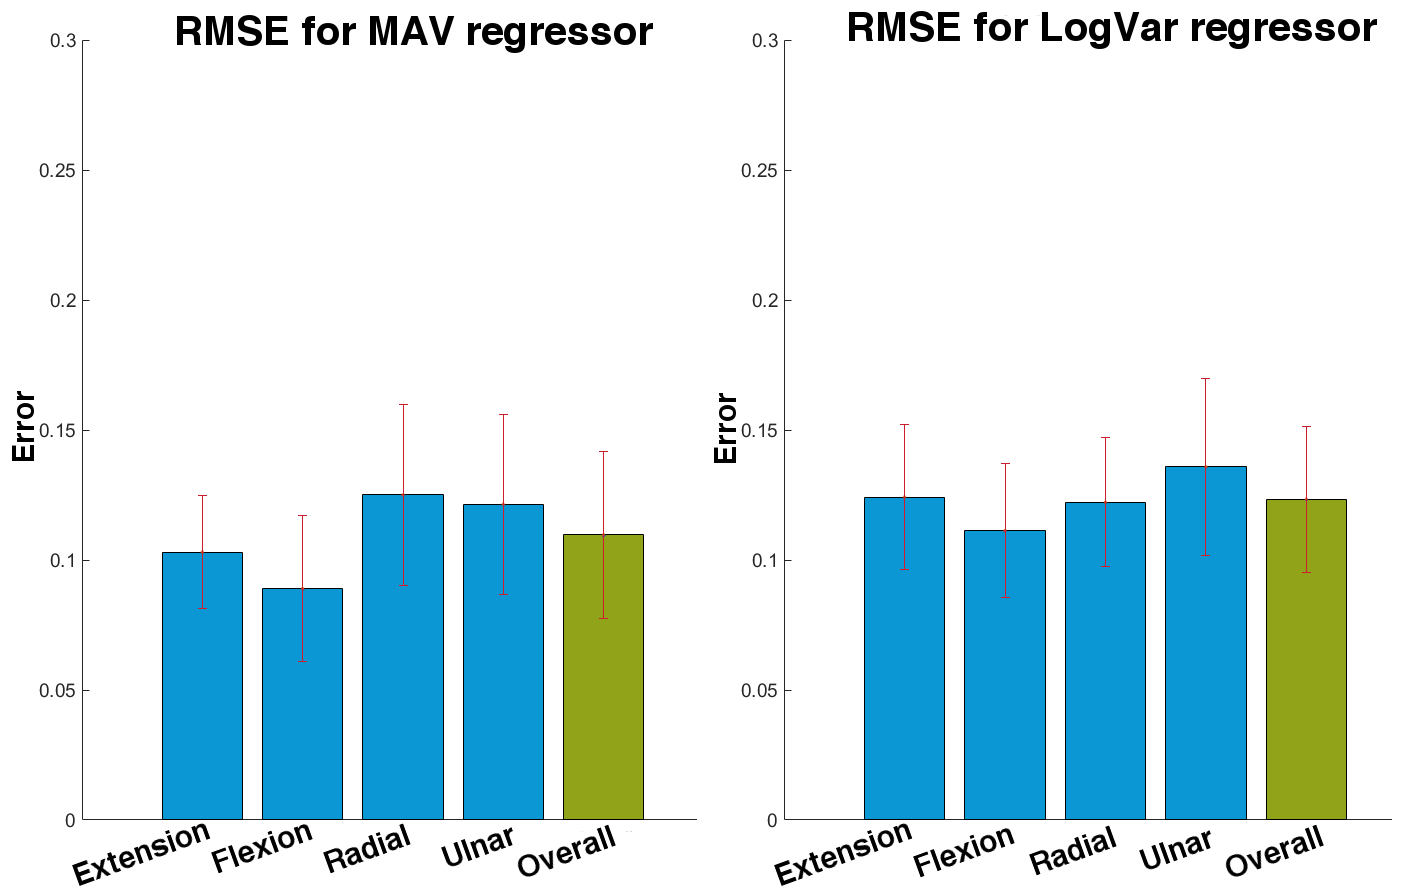
\includegraphics[scale=0.27]{figures/gimmeThemRMSEBars.png}
		\end{figure}
	Significant difference between MAV and LogVar (p = 0.0007)
\end{frame}

%\subsection{Offline Results}
\begin{frame}{Results}{Offline Results: test data}
\begin{figure}
	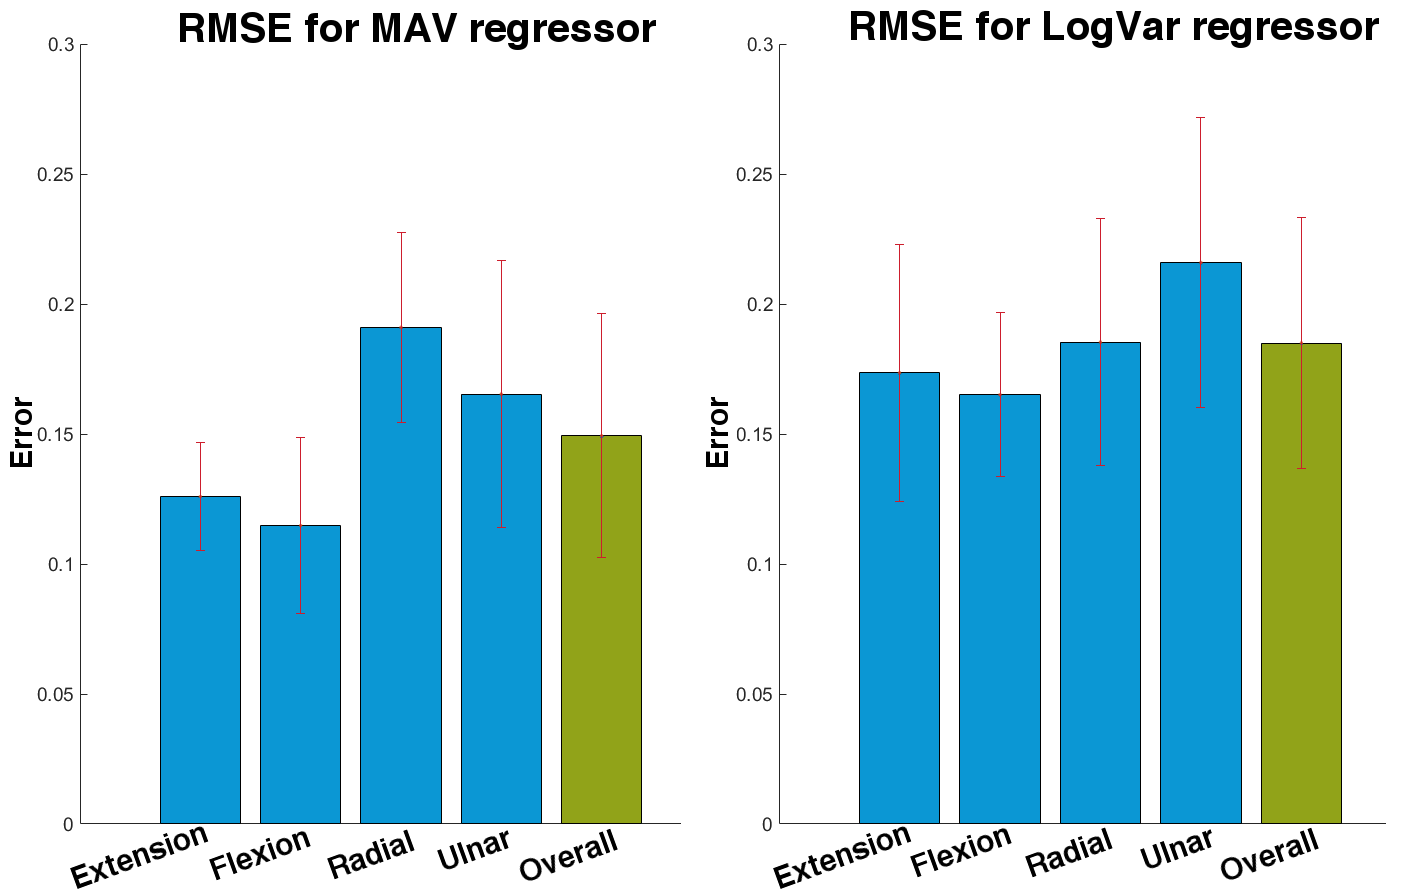
\includegraphics[scale=0.27]{figures/RMSEBarPlotNewData.png}
\end{figure}
Significant difference between MAV and LogVar (p = 0.00082)
\end{frame}

%\subsection{Offline Results}
\begin{frame}{Results}{Offline Results: training VS test}
\begin{itemize}
	\item Significant difference between MAV training and MAV test data (p = 0.0002)
	\item Significant difference between LogVar training and LogVar test data (p = 0.0002)
\end{itemize}
\end{frame}

%%% ONLINE RESULTS %%%

\subsection{Online Results}
\begin{frame}{Results}{Online Results: MAV}
\begin{figure}
	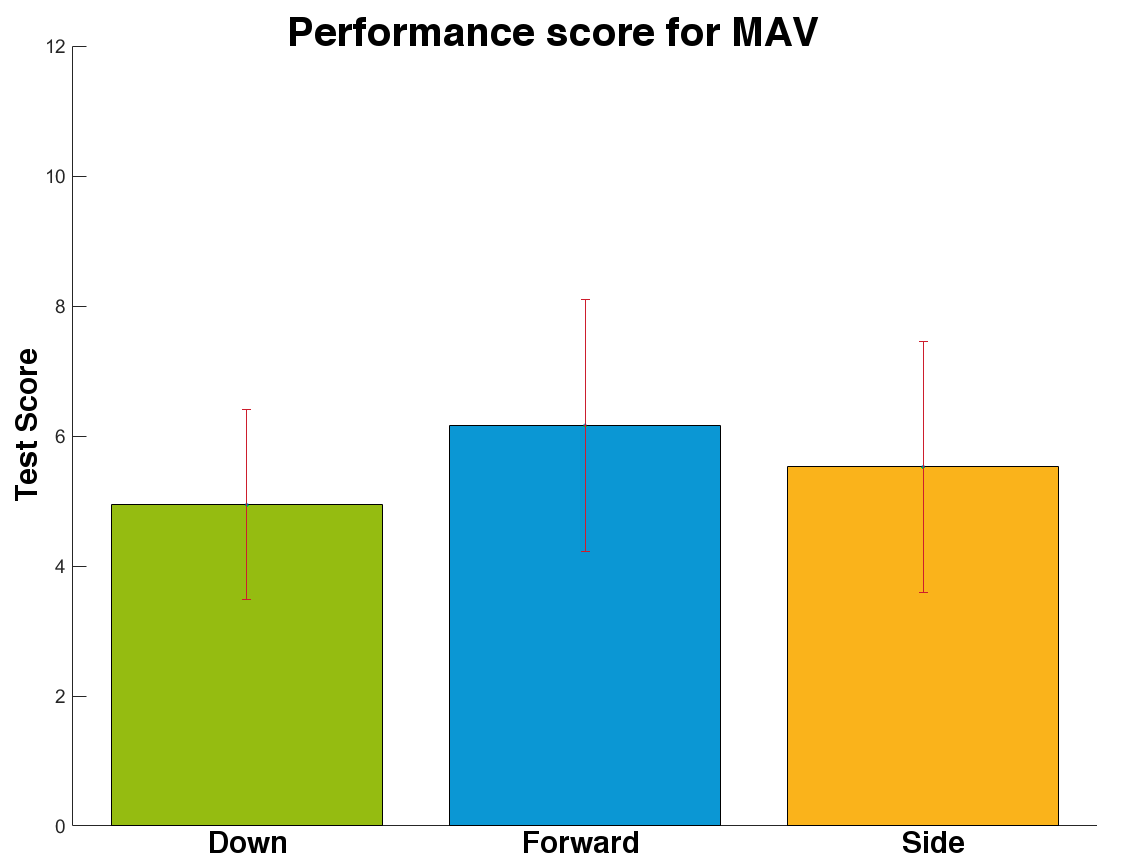
\includegraphics[scale=0.27]{figures/gotItMAV.png}
\end{figure}
No significant difference between limb positions (p = 0.16)
\end{frame}

%\subsection{Online Results}
\begin{frame}{Results}{Online Results: LogVar}
\begin{figure}
	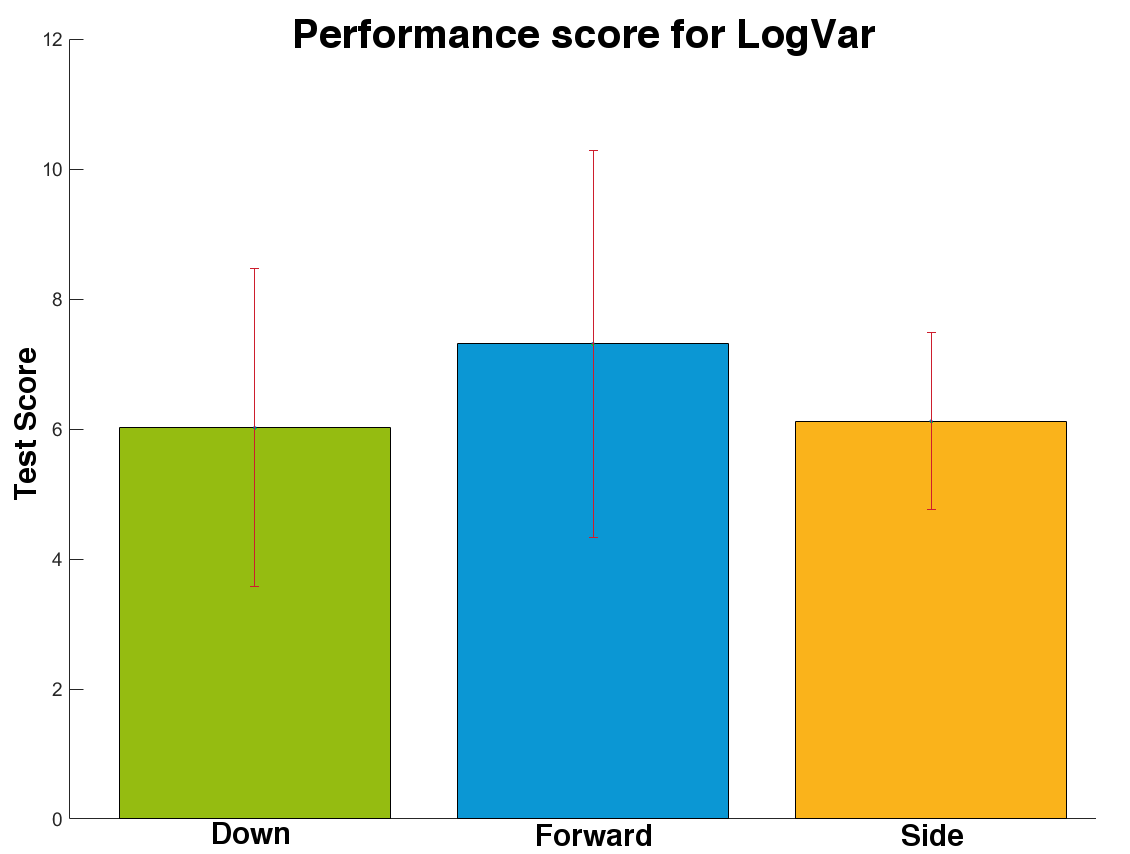
\includegraphics[scale=0.27]{figures/gotItLogVar.png}
\end{figure}
No significant difference between limb positions (p = 0.56)
\end{frame}

%\subsection{Online Results}
\begin{frame}{Results}{Online Results: feature comparison}
\begin{itemize}
	\item No significant difference between MAV and LogVar (p = 0.13)
\end{itemize}
\end{frame}


%%% DISCUSSION %%%

\section{Discussion}
% the license
\begin{frame}{Discussion}
\begin{itemize}
	\item<1-> No significant difference in performance across limb positions
	\item<2-> No correlation between offline and online test
	\item<3-> No significant difference in performance between the MAV and LogVar feature
	\item<4-> Large potential in linear regression-based myoelectric prosthetic control
\end{itemize}

\end{frame}



%%% ACKNOWLEDGEMENT %%%

\section{Acknowledgement}
% the license
\begin{frame}{Acknowledgement}
\begin{itemize}
	\item Supervisors: Strahinja Dosen, Jakob Dideriksen and Lotte Struijk
	\item SMH for providing equipment
	\item Test subjects and Mikkel Birkedal
\end{itemize}

\end{frame}


{\aauwavesbg
\begin{frame}[plain,noframenumbering]
  \finalpage{Thank you}
\end{frame}}
%%%%%%%%%%%%%%%%

\end{document}
